\cleardoublepage

\section{实验}
\subsection{实验环境}
总的来说,本次研究的实验是在Linux+Anaconda+Pytorch的环境下运行的。

Linux是一种自由和开放源码的类Unix操作系统,相较于另一个操作系统window,在Linux系统上运行神经网络有诸多优势。
首先是易用性强,window系统很多时候对硬件有较高要求,而Linux系统即使在低成本设备上也高度稳定;此外丰富且强大的
终端工具,使得我们执行效率大幅提升。其次是较快的配置速度,现阶段的深度学习个人开发环境依赖GPU,在Linux系统
上配置底层硬件,比window要容易快速得多。再者,是更好的生态,得益于Linux是一个开源的系统,它有更多深度学习框架
的官方支持,tensorflow,torch,docker等社区都是优先支持Linux。

Anaconda是一个免费开源的Python的发行版本,可以完成计算科学的各种任务。Anaconda主要解决了官方Python的两个问题。
其一,提供了强大的包管理功能,在数据分析中会使用很多第三方的包,conda(anaconda中的一个包管理器)可以为安装和
管理这些包提供帮助,包括安装、卸载和更新包。其二,提供了有效的环境管理功能,由于python版本的兼容
性问题,同时使用Python2和Python3容易造成许多混乱和错误,anaconda能够解决多版本Python并存、切换的问题。

Pytorch是一个GPU加速和自动求导的深度学习框架,可完成一些深度学习的任务。使用Pytorch主要出于两点考虑。一个方面是,
Pytorch使用动态图进行运算,和使用静态图计算的TensorFlow相比,动态图的运行机制更适合研究者调试。另一个方面是,Pytorch
的代码相对易写,pytorch的编码要求和python一致,可以像写python代码一样设计深度学习模型,而使用TensorFlow则要求使用
契合它的API,这相对来说比较复杂。

\subsection{数据集}
本次实验,我们的主要任务是节点级别的分类任务。对于一个给定的网络,我们已知它的图结构,它的部分节点已经被标记,部分节点未
被标记。图卷积神经网络可以通过学习一个鲁棒模型,来有效地识别未标记节点的类标记。为此,可以通过叠加一对图卷积层,然后再叠
加一个用于多分类的softmax层,来构建一个端到端的网络。如图4.1就展示了这样的例子。

本次研究使用当前比较流行的Cora、Citeseer、Pubmed数据集来进行实验,这三个数据集都是来自引文网络,主要任务是论文的分类(即
节点级分类的半监督学习)。引文网络就是由论文和他们的关系构成的网络,这些关系包括例如引用关系、共同的作者等,具有天然的图
结构。

以Cora数据集(图4.1)为例,Cora数据集由许多机器学习领域的论文构成,总共有2708篇论文,这些论文被分为7个类别。每一篇论文至少引用了
该数据集里面另外一篇论文或者被另外一篇论文所引用,原论文和引用的论文构成了一条天然的边,总共有5429条边。数据集中有一个包
含多个单词的词汇表,它去除了出现频率较小的词,最终词汇表中有1433个词汇,即每篇论文的特征维度是1433,然后论文中是否出现了
某个词用特征向量里值的0或1进行表示。我们实验默认已知5429条边(即已知图结构),且已知每篇论文的特征向量,知道部分论文的类别,
任务是对其他不知道类别的论文进行分类。

\begin{figure}[ht]
    \centering
    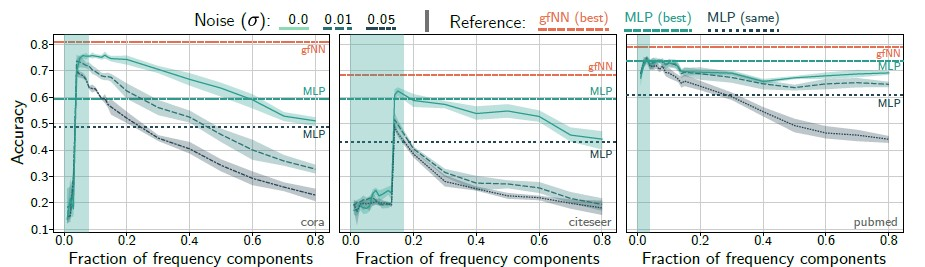
\includegraphics[width=4cm]{experiment/1.jpg}
    \caption{\label{4-1}Cora数据集可视化}
\end{figure}

\subsection{实验结果}
对比的三个神经网络分别是,GAT、our GAT、simple GAT,如图4.2所示。本部分将展示在Cora数据集上训练的实验结果,Citeseer和Pubmed
数据集的训练结果在附录1中,实验结果与Cora上类似。
\begin{figure}[ht]
    \centering
    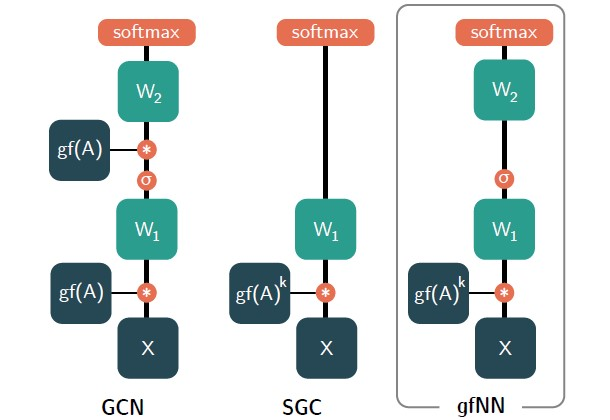
\includegraphics[width=6cm]{experiment/2.jpg}
    \caption{\label{4-2}神经网络结构图}
\end{figure}

\subsubsection{hop值的影响}
第一组实验,我们对比不同hop值的图结构对同一个神经网络的影响。考虑到不同的隐层特征维度会有不同的实现效果,
我们将隐层的特征维度选取为效果较好时的32和64,我们考察的方面为是否出现过拟合、每epoch的训练时间、分类的准确率。
结果见表4.1。

\begin{table}[]
    \centering
    \caption{不同的hop值对神经网络的影响}
    \begin{tabular}{|l|l|l|l|l|l|}
    \hline
                         & 图结构hop的值           & 隐层输出维度 & 过拟合 & 训练时间(ms)/epoch & 准确率      \\ \hline
    \multirow{4}{*}{GAT} & \multirow{2}{*}{1} & 32     & 不明显 & 0.39            & 82.2±0.5 \\ \cline{3-6}
                         &                    & 64     & 不明显 & 0.41            & 82.7±0.4 \\ \cline{2-6}
                         & \multirow{2}{*}{2} & 32     & 明显   & 1.05            & 77.7±1.5 \\ \cline{3-6}
                         &                    & 64     & 明显   & 1.10            & 78.5±1.2 \\ \hline
    \multirow{4}{*}{Simple GAT} & \multirow{2}{*}{1} & 32     & 不明显 & 0.19     & 80.1±0.3 \\ \cline{3-6}
                         &                    & 64     & 不明显 & 0.20            & 80.2±0.5 \\ \cline{2-6}
                         & \multirow{2}{*}{2} & 32     & 明显   & 0.42             & 78.1±1.0 \\ \cline{3-6}
                         &                    & 64     & 明显   & 0.59             & 77.6±0.9 \\ \hline                    
    \end{tabular}
\end{table}

通过分析实验结果,我们可以得到结论:GAT神经网络和Simple GAT神经网络,在图结构的hop值由1变为2时,会出现严重的过拟合现象,
并且训练时间边长,准确率下降。我们的实验也再次验证了,对于传统的GAT不能够通过增加hop值来提升图卷积神经网络的
表达能力。

更进一步地分析,为何hop值的增加会对实验效果产生负面的影响,原因大致分为以下两方面。一方面,是因为注意力矩阵$A$的非
零元素过多;当图结构的hop值为1时,$A$中的非零元素只包括一阶相连的边,而图结构的hop值为2时,$A$中的非零元素还包括二
阶相连的边;与hop为1时相比,过多的元素使得在训练注意力参数$ \vec{a} $的过程中,出现过拟合现象。另一个方面,节点间边
的相连表示了他们之间的联系,但可能数据集中并不是所有二阶相连的节点间都有明显的关系,所以注意力矩阵$A$中非零元素的冗余,
造成了过拟合。

\subsubsection{性能对比}
第二组,我们主要对比三种神经网络GAT、our GAT、simple GAT的性能。我们依旧将隐层的特征维度选取为32和64,考察的方面为
是否出现过拟合、每epoch的训练时间、分类的准确率。由第三章我们易知,当our GAT的hop值取1时,结构上等同于simple GAT网络。
所以在本组实验中,我们将GAT和Simple GAT的hop值选取为1,将Our GAT的hop值选取为2。结果见表4.2。

\begin{table}[]
    \centering
    \caption{三种神经网络效果对比}
    \begin{tabular}{|l|l|l|l|l|l|}
    \hline
                                & 图结构hop的值           & 隐层输出维度 & 过拟合 & 训练时间(ms)/epoch & 准确率      \\ \hline
    \multirow{2}{*}{GAT}        & \multirow{2}{*}{1} & 32     & 不明显 & 0.39           & 82.2±0.5 \\ \cline{3-6} 
                                &                    & 64     & 不明显 & 0.41           & 82.7±0.4 \\ \hline
    \multirow{2}{*}{Simple GAT} & \multirow{2}{*}{1} & 32     & 不明显 & 0.19           & 80.1±0.3 \\ \cline{3-6} 
                                &                    & 64     & 不明显 & 0.20           & 80.2±0.5 \\ \hline
    \multirow{2}{*}{Our GAT}    & \multirow{2}{*}{2} & 32     & 不明显 & 0.20           & 82.4±0.6 \\ \cline{3-6} 
                                &                    & 64     & 不明显 & 0.20           & 82.5±0.5 \\ \hline
    \end{tabular}
\end{table}

实验结果表明了:我们提出的图卷积神经网络our GAT,在测试数据集上的准确率大致与传统GAT网络持平,但我们的训练效率较其提升了一倍,
训练效率大致等同于simple GAT;此外,实验过程中,我们提出的our GAT的hop值设置为2,并没有出现过拟合现象,这说明其克服了传统GAT网络
hop值只能为1的缺陷。

我们的设计思路上在实验结果上得到了验证。与GAT和simple GAT直接增加注意力矩阵$A$的hop值相比,在our GAT的神经网络结构下,
$A$hop值依然为1,我们通过矩阵多项式$ F(A) $来间接地增加图结构的hop。正是这样的设计,使得我们在几乎不影响simple GAT网络训练效率
的情况下,大大增加了其表达能力,也成功避免了过拟合;也正是因为矩阵多项式带来的表达能力的提升,我们能够将传统GAT网络中使用的两个
注意力矩阵$ A_1,A_2 $减少为一个,在不影响训练效果的前提下,增加了其训练速度。

\subsubsection{hop值的选取}

